%%%%%%%%%%%%%%%%%%%%%%%%%%%%%%%%%%%%%%%%%%%%%%%%%%%%%%%%%%%
% ImageLib Technical Report - Rho-class Template
%%%%%%%%%%%%%%%%%%%%%%%%%%%%%%%%%%%%%%%%%%%%%%%%%%%%%%%%%%%

\documentclass[9pt,a4paper,twocolumn,twoside]{rho-class/rho}
\usepackage[english]{babel}

%----------------------------------------------------------
% Title
%----------------------------------------------------------

\doctype{Technical Report}
\title{ImageLib: A High-Performance C++ Image Processing Library with CUDA GPU Acceleration}

%----------------------------------------------------------
% Authors, Affiliations and dates
%----------------------------------------------------------

\author[{\textasteriskcentered},a,1]{Ziheng Fan}

%----------------------------------------------------------

\affil[a]{Department of Computer Science}

%----------------------------------------------------------

\dates{This manuscript was compiled on \today}

%----------------------------------------------------------
% Corresponding author-, Document- information
%----------------------------------------------------------

\corres{\textsuperscript{\textasteriskcentered}Developer and Author.}

%----------------------------------------------------------

\docinfo{Built with Visual Studio 2022 (v145), CUDA Toolkit 12.4, and tested on NVIDIA RTX 4060 Laptop GPU. Source code available at: \texttt{D:\textbackslash Github\textbackslash VStest}.}

%----------------------------------------------------------

\journalname{Visual Studio C++ Project}
\journal{ImageLib v1.0 -- 2026}
\theday{\today}
\vol{1}
\no{1}

%----------------------------------------------------------
% Abstract and Keywords
%----------------------------------------------------------

\begin{abstract}
    This report presents \textbf{ImageLib}, a comprehensive C++ image processing library featuring over 4,500 lines of modern C++20 code organized into a multi-project Visual Studio solution. The library provides a complete image processing pipeline covering color space conversions, spatial filtering (convolution, Gaussian blur, bilateral filter, median filter), geometric transformations (resize, rotate, affine/perspective), edge detection (Sobel, Canny), morphological operations, histogram analysis, feature detection (Harris corners, FAST, Hough lines), and a plugin architecture. A key contribution is the \textbf{CUDA GPU acceleration module} (CudaLib), which offloads compute-intensive operations to the GPU using shared memory tiling, constant memory kernels, and histogram-based parallel algorithms. Benchmarks on an NVIDIA RTX 4060 Laptop GPU demonstrate speedups ranging from \textbf{6.6$\times$} (invert) to \textbf{1,441$\times$} (Sobel edge detection) compared to CPU-only execution, with bilateral filtering achieving \textbf{626$\times$} and median filtering \textbf{754$\times$} acceleration.
\end{abstract}

%----------------------------------------------------------

\keywords{Image Processing, CUDA, GPU Acceleration, C++20, Computer Vision, Convolution, Edge Detection}

%----------------------------------------------------------

\begin{document}

    \maketitle
    \thispagestyle{firststyle}

%----------------------------------------------------------

\section{Introduction}

    \rhostart{I}mage processing is a fundamental component of computer vision, medical imaging, remote sensing, and multimedia applications \cite{gonzalez2018digital}. While many established libraries exist (OpenCV, ITK), building one from scratch provides deep understanding of algorithmic design, memory management, and hardware acceleration strategies.

    This project implements \textbf{ImageLib}, a self-contained C++ image processing library with no external dependencies beyond the C++ standard library and CUDA Toolkit. The goals are threefold:

    \begin{enumerate}
        \item Provide a \textbf{complete} image processing toolkit covering I/O, color manipulation, filtering, transforms, feature detection, and morphological operations.
        \item Demonstrate \textbf{modern C++20} \cite{cpp20standard} design patterns including template metaprogramming, move semantics, RAII, and lambda-based pipelines.
        \item Achieve \textbf{massive performance gains} through CUDA GPU acceleration \cite{cuda-toolkit}, with a clean separation between CPU and GPU code paths.
    \end{enumerate}

    The solution comprises four Visual Studio projects: \texttt{ImageLib} (core static library), \texttt{CudaLib} (GPU kernels), \texttt{ImageDemo} (demonstration application), and \texttt{Tests} (unit test suite with 80+ test cases).

\section{System Architecture}

    \subsection{Project Structure}

        The solution follows a layered architecture with clear separation of concerns:

        \begin{itemize}
            \item \textbf{ImageLib} (15 headers, 8 source files) -- Pure C++ static library containing all image processing algorithms and the \texttt{GpuAccel} dispatch layer.
            \item \textbf{CudaLib} (2 headers, 10 \texttt{.cu} files) -- CUDA static library compiled with \texttt{nvcc}, containing all GPU kernel implementations.
            \item \textbf{ImageDemo} -- Console application exercising all features with timing benchmarks.
            \item \textbf{Tests} -- Custom test framework with 80+ unit tests covering every module.
        \end{itemize}

    \subsection{Core Image Class}

        The central abstraction is a template class \texttt{Image<PixelT>} supporting arbitrary pixel types:

        \begin{itemize}
            \item \texttt{ImageRGB} -- 3-channel \texttt{uint8\_t} (24-bit color)
            \item \texttt{ImageGray} -- Single-channel \texttt{uint8\_t}
            \item \texttt{ImageF} -- Single-channel \texttt{float}
            \item \texttt{ImageRGBA} -- 4-channel with alpha
        \end{itemize}

        The class uses contiguous row-major memory layout via \texttt{std::unique\_ptr<PixelT[]>}, enabling direct \texttt{cudaMemcpy} compatibility. It supports move semantics, border-aware sampling (Zero, Clamp, Reflect, Wrap), region-of-interest extraction, and Bresenham-based drawing primitives.

        \figref{fig:drawing} demonstrates the drawing primitives rendered by the \texttt{Image} class, including lines, circles, and rectangles computed via Bresenham's algorithm and the midpoint circle method.

        \begin{figure}[H]
            \centering
            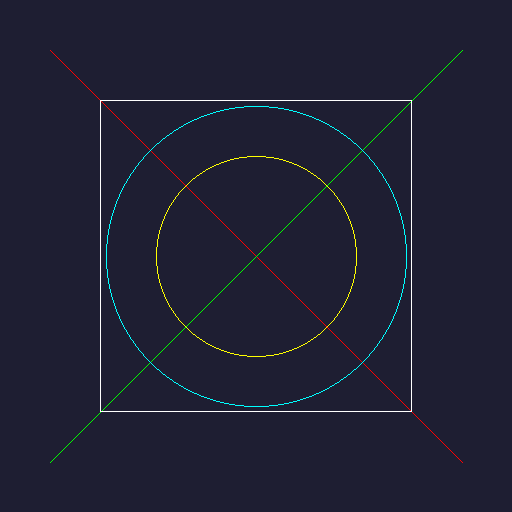
\includegraphics[width=0.65\columnwidth]{figures/drawing.png}
            \caption{Drawing primitives: lines, circles, and rectangles rendered by the \texttt{Image} class using Bresenham's algorithm.}
            \label{fig:drawing}
        \end{figure}

\section{CPU Image Processing Modules}

    \subsection{Procedural Image Generation}

        The library includes several procedural generators for testing: Mandelbrot fractals, Perlin noise, checkerboards, and multi-corner gradients. \figref{fig:procedural} shows representative outputs.

        \begin{figure}[H]
            \centering
            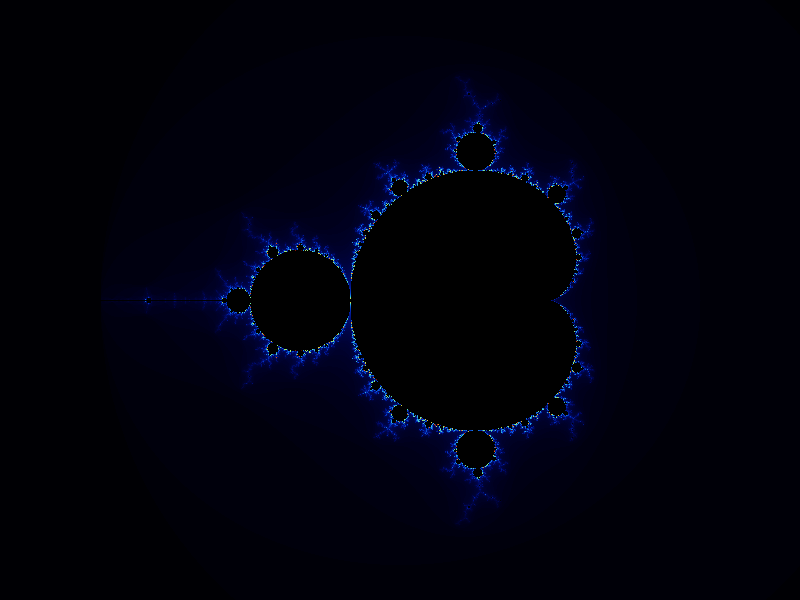
\includegraphics[width=0.48\columnwidth]{figures/mandelbrot.png}
            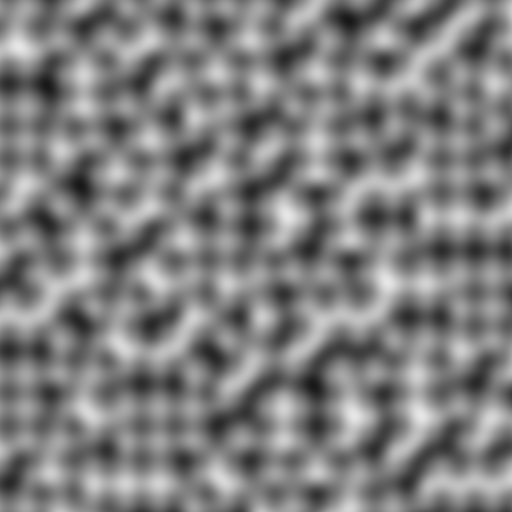
\includegraphics[width=0.48\columnwidth]{figures/perlin.png}
            \caption{Procedural generation: Mandelbrot fractal (left, 800$\times$600) and Perlin noise (right, 512$\times$512).}
            \label{fig:procedural}
        \end{figure}

    \subsection{Color Space Conversions}

        The \texttt{ColorSpace} module supports bidirectional conversions between RGB, HSV, HSL, and YCbCr color spaces. Image-level operations include brightness, contrast, saturation, hue rotation, gamma correction, inversion, sepia tone, posterization, and solarization. Otsu's method \cite{otsu1979threshold} provides automatic threshold selection for binarization. \figref{fig:color} illustrates several color operations.

        \begin{figure}[H]
            \centering
            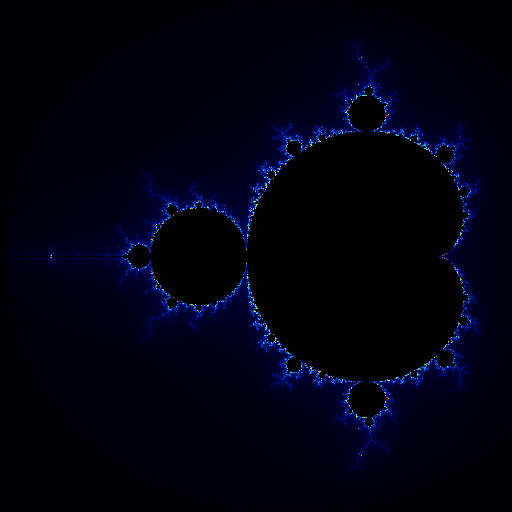
\includegraphics[width=0.32\columnwidth]{figures/source.png}
            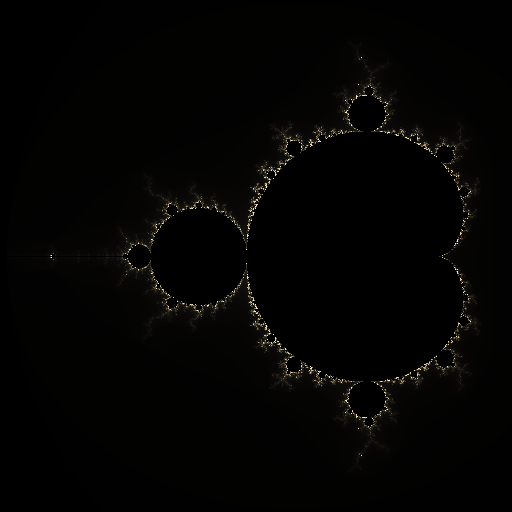
\includegraphics[width=0.32\columnwidth]{figures/sepia.png}
            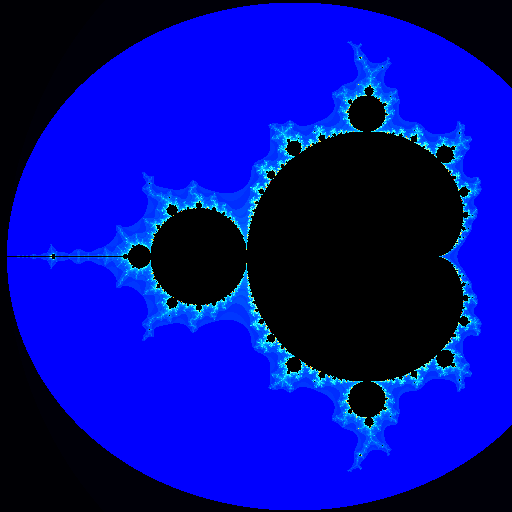
\includegraphics[width=0.32\columnwidth]{figures/equalized.png}
            \caption{Color operations on the source image: original (left), sepia tone (center), and histogram equalization (right).}
            \label{fig:color}
        \end{figure}

    \subsection{Spatial Filtering}

        The \texttt{Filter} module implements both linear and non-linear filters:

        \begin{itemize}
            \item \textbf{Convolution} -- Generic 2D convolution with configurable border handling. Predefined kernels include Gaussian, Sobel, Prewitt, Laplacian, Laplacian-of-Gaussian, Sharpen, Emboss, and Unsharp Mask.
            \item \textbf{Separable convolution} -- Two-pass optimization reducing $O(K^2)$ to $O(2K)$ per pixel for separable kernels.
            \item \textbf{Median filter} -- Uses \texttt{std::nth\_element} for $O(n \log n)$ per-pixel sorting.
            \item \textbf{Bilateral filter} -- Edge-preserving smoothing with spatial and range Gaussian weighting \cite{tomasi1998bilateral}.
        \end{itemize}

        \figref{fig:filters} demonstrates Gaussian blur and noise removal via median filtering.

        \begin{figure}[H]
            \centering
            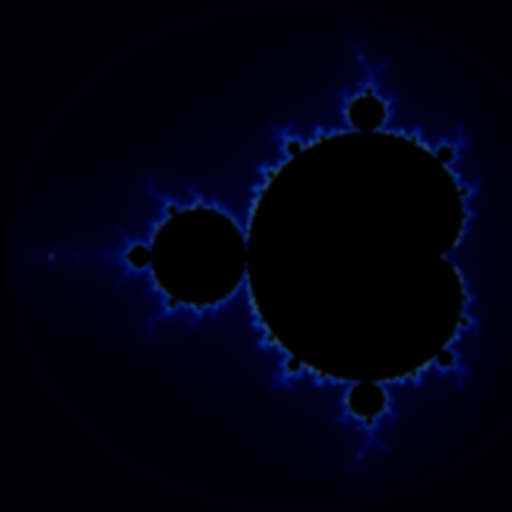
\includegraphics[width=0.48\columnwidth]{figures/gaussian_blur.png}
            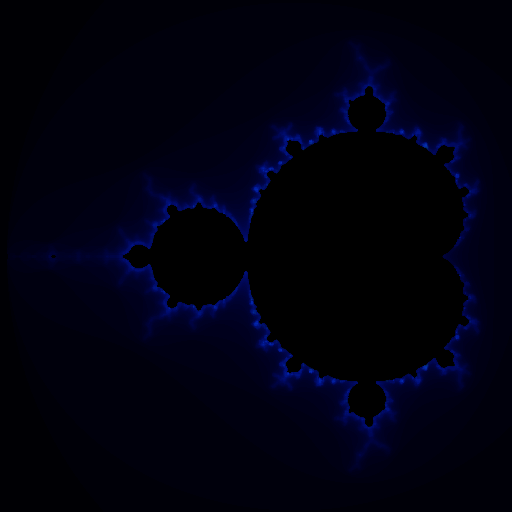
\includegraphics[width=0.48\columnwidth]{figures/median.png}
            \caption{Spatial filtering: Gaussian blur $r$=5 (left) and median filter $r$=2 (right).}
            \label{fig:filters}
        \end{figure}

        \figref{fig:denoise} shows salt-and-pepper noise addition and subsequent denoising with a median filter.

        \begin{figure}[H]
            \centering
            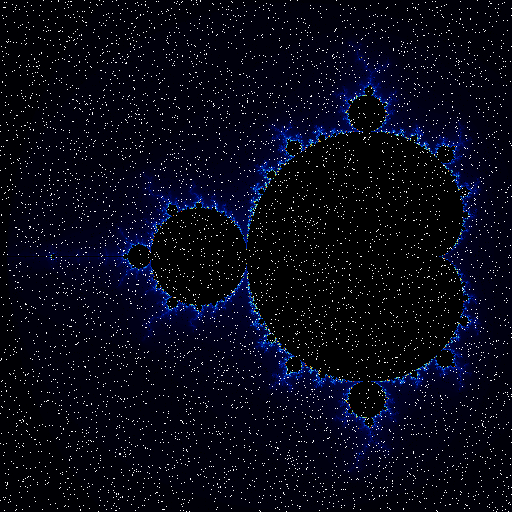
\includegraphics[width=0.48\columnwidth]{figures/salt_pepper.png}
            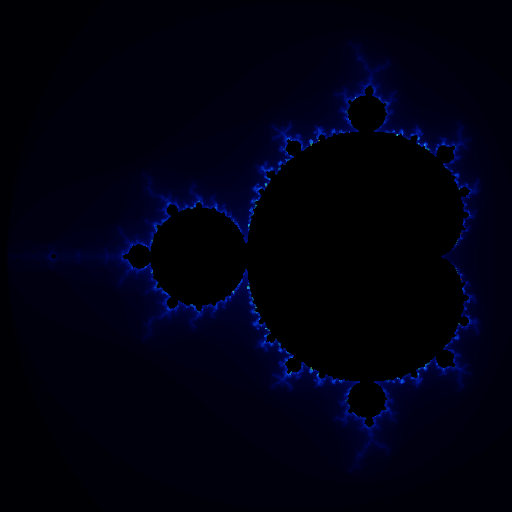
\includegraphics[width=0.48\columnwidth]{figures/denoised.png}
            \caption{Noise removal: 5\% salt-and-pepper noise (left) cleaned by median filter (right).}
            \label{fig:denoise}
        \end{figure}

    \subsection{Edge Detection}

        The library implements multiple edge detection algorithms. The Canny edge detector \cite{canny1986computational} provides a full pipeline: Gaussian blur, Sobel gradient computation, non-maximum suppression, double thresholding, and hysteresis edge tracking. \figref{fig:edges} compares Sobel and Canny results.

        \begin{figure}[H]
            \centering
            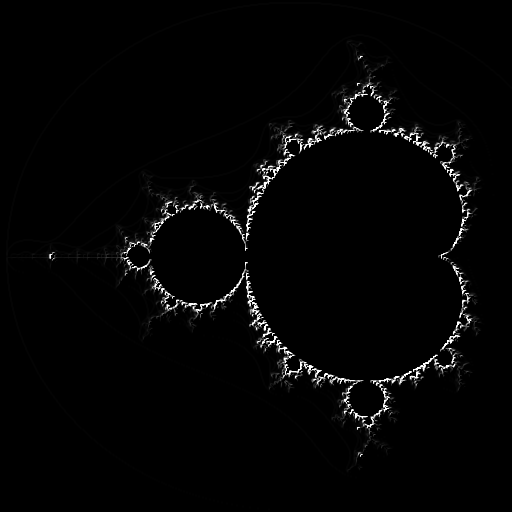
\includegraphics[width=0.48\columnwidth]{figures/sobel.png}
            
\includegraphics[width=0.48\columnwidth]{figures/canny.png}
            \caption{Edge detection: Sobel magnitude (left) and Canny edge detector (right).}
            \label{fig:edges}
        \end{figure}

    \subsection{Geometric Transformations}

        Supported operations include flip, rotation (90\textdegree/180\textdegree/arbitrary angle), resize with nearest-neighbor/bilinear/bicubic interpolation, crop, padding, affine transforms (with matrix composition and inversion), and distortion effects. \figref{fig:distort} shows the swirl distortion effect.

        \begin{figure}[H]
            \centering
            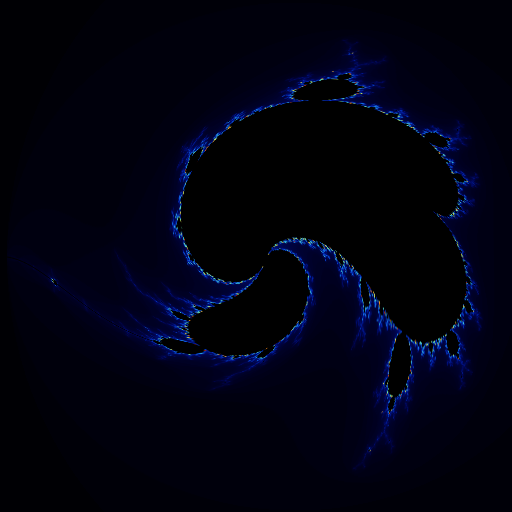
\includegraphics[width=0.65\columnwidth]{figures/swirl.png}
            \caption{Swirl distortion effect with angle $= 3.0$ radians applied to the source image.}
            \label{fig:distort}
        \end{figure}

    \subsection{Histogram Analysis}

        The \texttt{Histogram} module computes per-channel histograms with statistical measures (mean, standard deviation, entropy, median, mode). Operations include histogram equalization, contrast stretching, and histogram matching. \figref{fig:histogram} shows a computed RGB histogram.

        \begin{figure}[H]
            \centering
            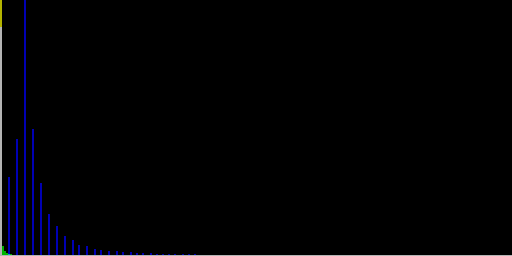
\includegraphics[width=0.75\columnwidth]{figures/histogram_rgb.png}
            \caption{RGB histogram visualization of the source image, rendered with per-channel color overlays.}
            \label{fig:histogram}
        \end{figure}

    \subsection{Feature Detection}

        Implemented algorithms include Harris corner detection \cite{harris1988combined} with non-maximum suppression, FAST corner detection \cite{rosten2006machine} (FAST-9 with score ranking), connected component labeling (union-find), blob detection with circularity filtering, and Hough line detection \cite{hough1962method}. \figref{fig:features} shows detected Harris corners overlaid on the source image.

        \begin{figure}[H]
            \centering
            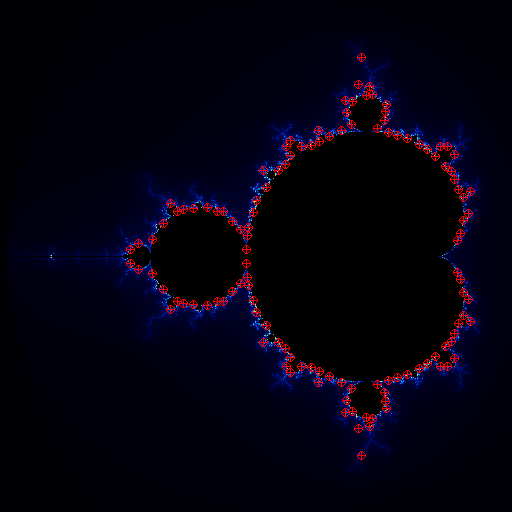
\includegraphics[width=0.65\columnwidth]{figures/harris.png}
            \caption{Harris corner detection: 126 corners detected with non-maximum suppression (radius=5, $k$=0.04). Red crosshairs mark detected corners.}
            \label{fig:features}
        \end{figure}

    \subsection{Morphological Operations}

        Binary and grayscale morphology includes erode, dilate, opening, closing, morphological gradient, top-hat, black-hat, skeletonization, distance transform, flood fill, and boundary extraction. \figref{fig:morph} compares erosion and dilation results.

        \begin{figure}[H]
            \centering
            
\includegraphics[width=0.48\columnwidth]{figures/erode.png}
            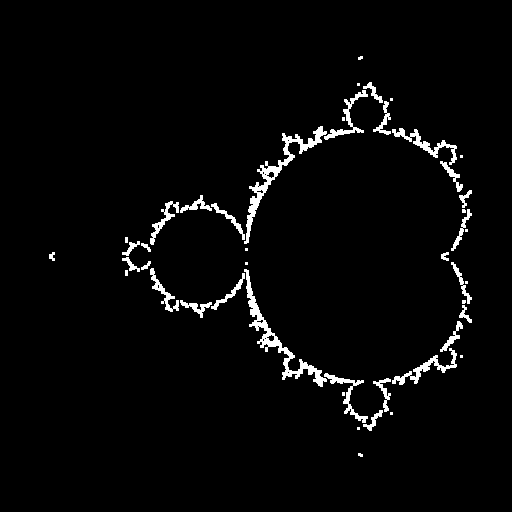
\includegraphics[width=0.48\columnwidth]{figures/dilate.png}
            \caption{Morphological operations on the binarized source: erosion (left) and dilation (right) with a 3$\times$3 rectangular structuring element.}
            \label{fig:morph}
        \end{figure}

\section{CUDA GPU Acceleration}

    \subsection{Architecture}

        GPU acceleration follows a \textbf{dispatch pattern}: the \texttt{GpuAccel.h} header in ImageLib declares GPU-accelerated function signatures mirroring the CPU API. When compiled with \texttt{IMAGELIB\_HAS\_CUDA}, these functions upload data to GPU via \texttt{GpuBuffer<T>}, invoke CUDA kernels from CudaLib, and download results. Without CUDA, stub implementations throw exceptions.

        The \texttt{GpuBuffer<T>} class manages device memory with RAII semantics (move-only, automatic \texttt{cudaFree} on destruction), and provides \texttt{uploadFrom}/\texttt{downloadTo}/\texttt{toImage} methods leveraging the contiguous memory layout of \texttt{Image<T>}.

    \subsection{Kernel Optimization Strategies}

        Following established GPU programming practices \cite{kirk2016programming}, the following optimization strategies are employed:

        \begin{itemize}
            \item \textbf{Shared memory tiling} -- Convolution kernels load image tiles plus halo regions into shared memory, reducing global memory accesses from $O(K^2)$ to $O(1)$ per thread after the initial cooperative load.
            \item \textbf{Constant memory} -- Convolution weights are stored in \texttt{\_\_constant\_\_} memory (64 KB, cached), providing broadcast-efficient read access across all threads.
            \item \textbf{Separable decomposition} -- Gaussian blur uses two-pass horizontal/vertical kernels with independent shared memory loading.
            \item \textbf{Fast math intrinsics} -- Bilateral filter uses \texttt{\_\_expf()} for hardware-accelerated exponential computation.
            \item \textbf{Histogram-based median} -- Instead of sorting, each thread builds a local 256-bin histogram and scans for the median, achieving $O(K^2 + 256)$ complexity per pixel.
            \item \textbf{Atomic shared memory} -- Histogram computation uses per-block \texttt{atomicAdd} in shared memory, followed by a reduction kernel to merge block-level histograms.
            \item \textbf{Iterative hysteresis} -- Canny edge detection implements the hysteresis step as repeated kernel launches with a device-side convergence flag.
        \end{itemize}

    \subsection{Implemented GPU Operations}

        \tabref{tab:gpuops} lists all GPU-accelerated operations and their kernel configurations.

        \begin{table}[H]
            \caption{CUDA Kernel Implementations}
            \label{tab:gpuops}
            \begin{tabular}{
                >{\raggedright\arraybackslash}p{0.32\columnwidth}
                >{\raggedright\arraybackslash}p{0.32\columnwidth}
                >{\raggedright\arraybackslash}p{0.22\columnwidth}
            }
            \toprule
            \textbf{Operation} & \textbf{Optimization} & \textbf{Block Size} \\
            \midrule
            2D Convolution & Shared mem tiling & 16$\times$16 \\
            Separable Conv. & Two-pass, shared mem & 256$\times$1 \\
            Bilateral Filter & \texttt{\_\_expf()}, const mem & 16$\times$16 \\
            Median Filter & Histogram-based & 16$\times$16 \\
            Resize (bilinear) & Per-pixel independent & 16$\times$16 \\
            Resize (bicubic) & 4$\times$4 tap weights & 16$\times$16 \\
            Histogram & Shared atomics & 256$\times$1 \\
            Sobel / Canny & Gradient + NMS + hyst. & 16$\times$16 \\
            Erode / Dilate & Min/Max over window & 16$\times$16 \\
            Color ops & Per-pixel map & 256$\times$1 \\
            \bottomrule
            \end{tabular}
        \end{table}

    \subsection{GPU Output Verification}

        \figref{fig:gpuoutput} shows GPU-processed images compared with CPU output to verify visual correctness.

        \begin{figure}[H]
            \centering
            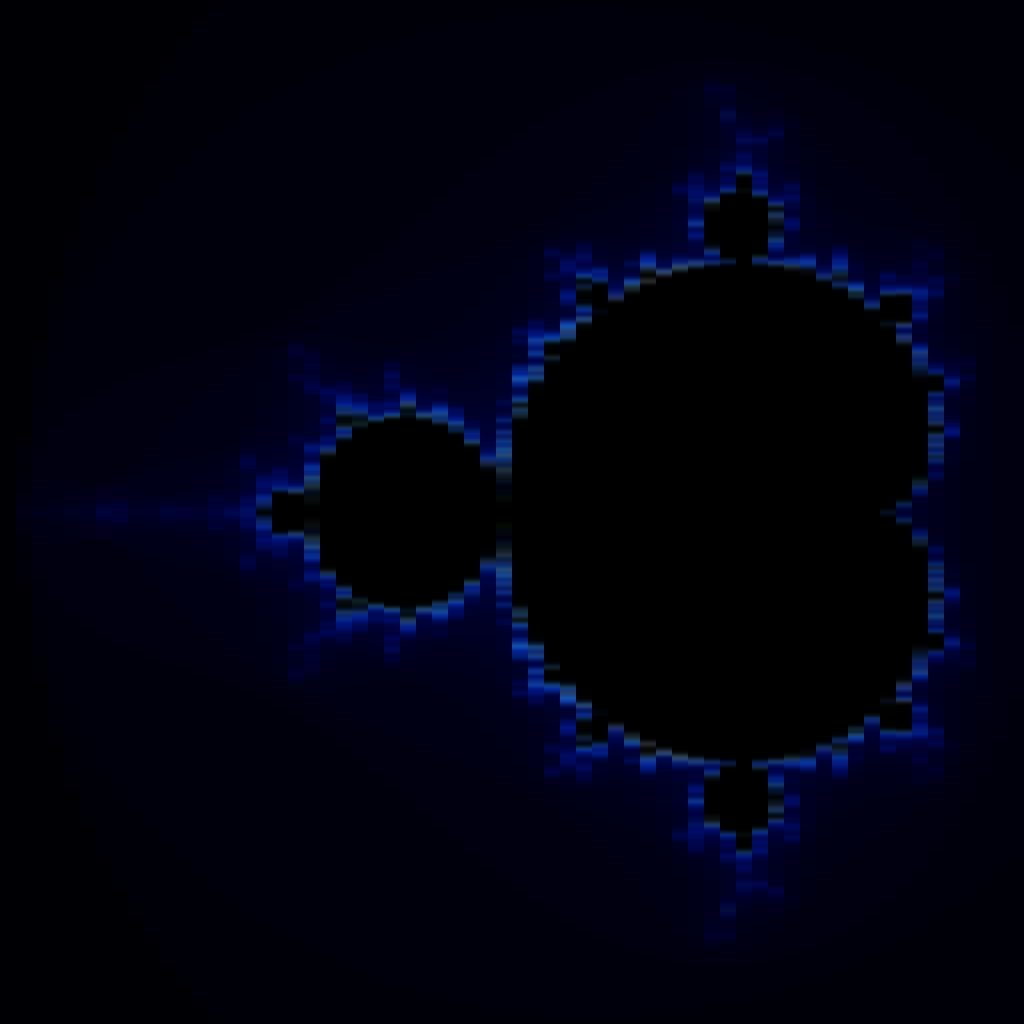
\includegraphics[width=0.48\columnwidth]{figures/gpu_gaussian.png}
            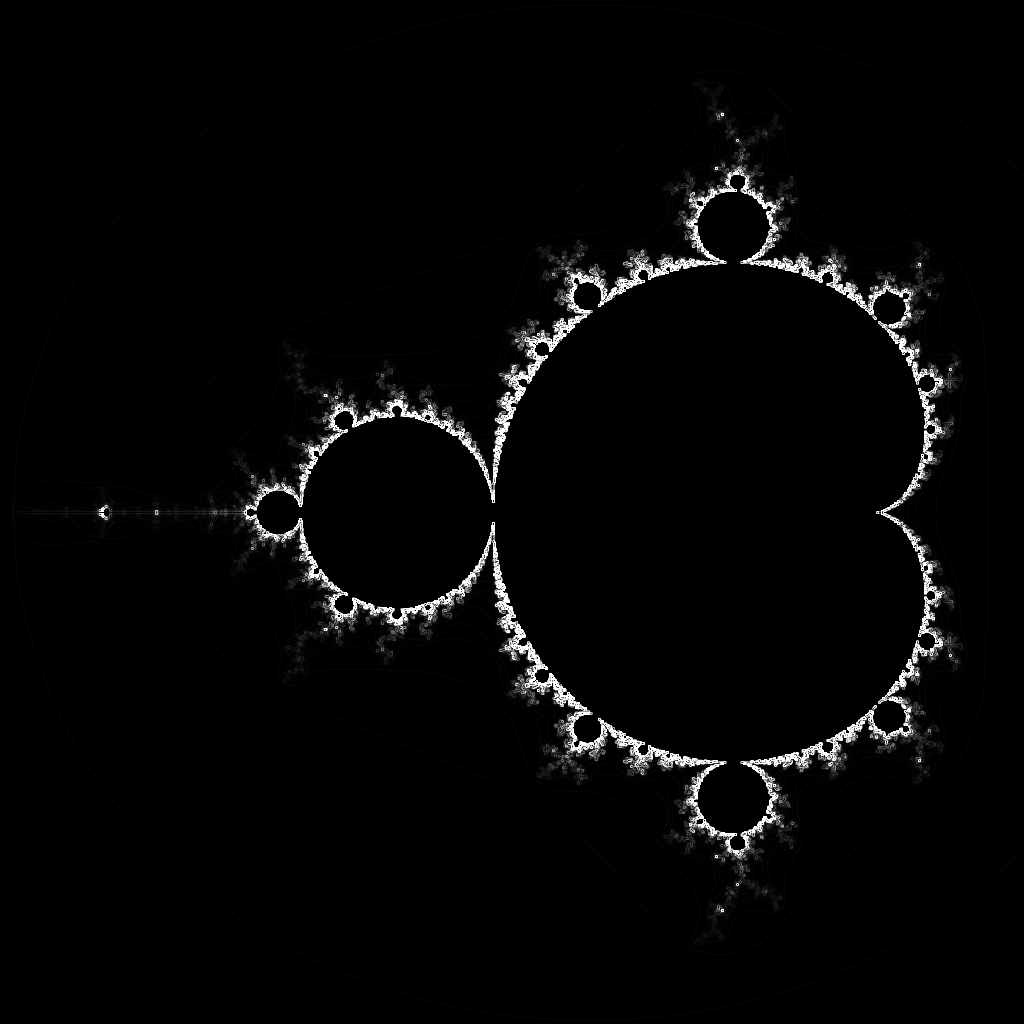
\includegraphics[width=0.48\columnwidth]{figures/gpu_sobel.png}
            \caption{GPU-accelerated results on 1024$\times$1024 images: Gaussian blur $r$=5 (left) and Sobel edge detection (right), visually identical to CPU output.}
            \label{fig:gpuoutput}
        \end{figure}

        \begin{figure}[H]
            \centering
            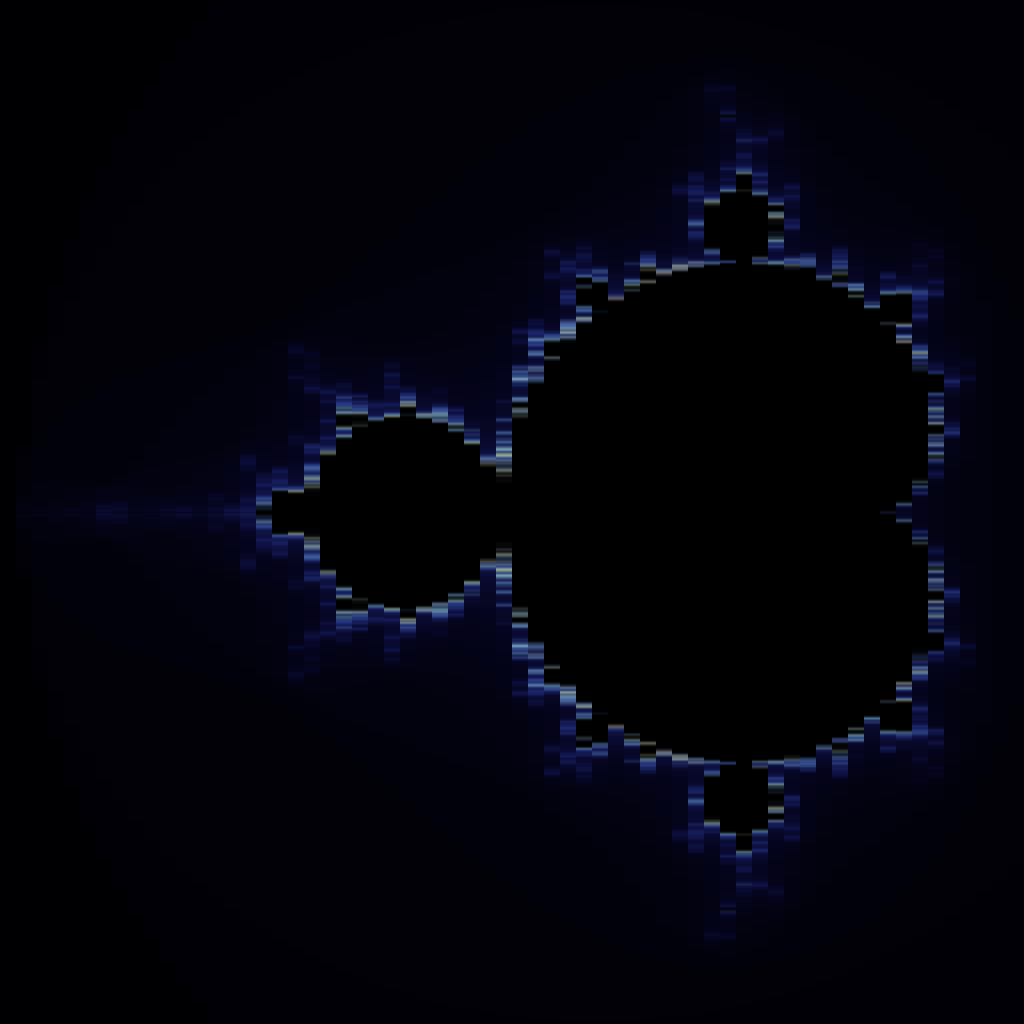
\includegraphics[width=0.65\columnwidth]{figures/gpu_pipeline.png}
            \caption{GPU pipeline output: brightness $\rightarrow$ contrast $\rightarrow$ Gaussian blur $\rightarrow$ sepia, completed in 36 ms total.}
            \label{fig:gpupipeline}
        \end{figure}

\section{Experimental Results}

    \subsection{Test Environment}

        All benchmarks were conducted on the following hardware:

        \begin{itemize}
            \item \textbf{CPU}: 24-thread processor (via \texttt{std::thread::hardware\_concurrency})
            \item \textbf{GPU}: NVIDIA GeForce RTX 4060 Laptop GPU (Ada Lovelace, SM 8.9, 8 GB VRAM)
            \item \textbf{CUDA}: Toolkit 12.4, compiled with \texttt{compute\_89, sm\_89}
            \item \textbf{Compiler}: MSVC v14.50 (v145), C++20, AVX2 enabled
            \item \textbf{OS}: Windows 11 Pro
        \end{itemize}

    \subsection{GPU vs CPU Benchmark}

        \tabref{tab:benchmark} presents the performance comparison on a 1024$\times$1024 test image (Mandelbrot fractal). \figref{fig:benchmark} visualizes the timing data on a logarithmic scale.

        \begin{table}[H]
            \caption{CPU vs GPU Performance (1024$\times$1024 image)}
            \label{tab:benchmark}
            \begin{tabular}{
                >{\raggedright\arraybackslash}p{0.30\columnwidth}
                >{\raggedright\arraybackslash}p{0.18\columnwidth}
                >{\raggedright\arraybackslash}p{0.18\columnwidth}
                >{\raggedright\arraybackslash}p{0.17\columnwidth}
            }
            \toprule
            \textbf{Operation} & \textbf{CPU (ms)} & \textbf{GPU (ms)} & \textbf{Speedup} \\
            \midrule
            Sobel Edge & 2713.0 & 1.88 & 1441$\times$ \\
            Erode 5$\times$5 & 3509.2 & 2.66 & 1319$\times$ \\
            Dilate 5$\times$5 & 3234.1 & 2.51 & 1290$\times$ \\
            Median $r$=2 & 23912.5 & 31.71 & 754$\times$ \\
            Bilateral $r$=5 & 15717.8 & 25.12 & 626$\times$ \\
            Gaussian $r$=5 & 2800.8 & 17.41 & 161$\times$ \\
            Convolution 5$\times$5 & 1247.2 & 10.28 & 121$\times$ \\
            Resize 2048$^2$ & 3305.2 & 33.93 & 97$\times$ \\
            Contrast $\times$1.5 & 281.7 & 8.34 & 34$\times$ \\
            Brightness +50 & 229.5 & 9.58 & 24$\times$ \\
            Hist.\ Equalize & 69.0 & 2.97 & 23$\times$ \\
            Grayscale & 31.0 & 2.52 & 12$\times$ \\
            Invert & 68.7 & 10.46 & 7$\times$ \\
            \bottomrule
            \end{tabular}
            \tabletext{GPU timings include host-to-device and device-to-host transfer overhead. Measured in Debug configuration.}
        \end{table}

        \begin{figure}[H]
            \centering
            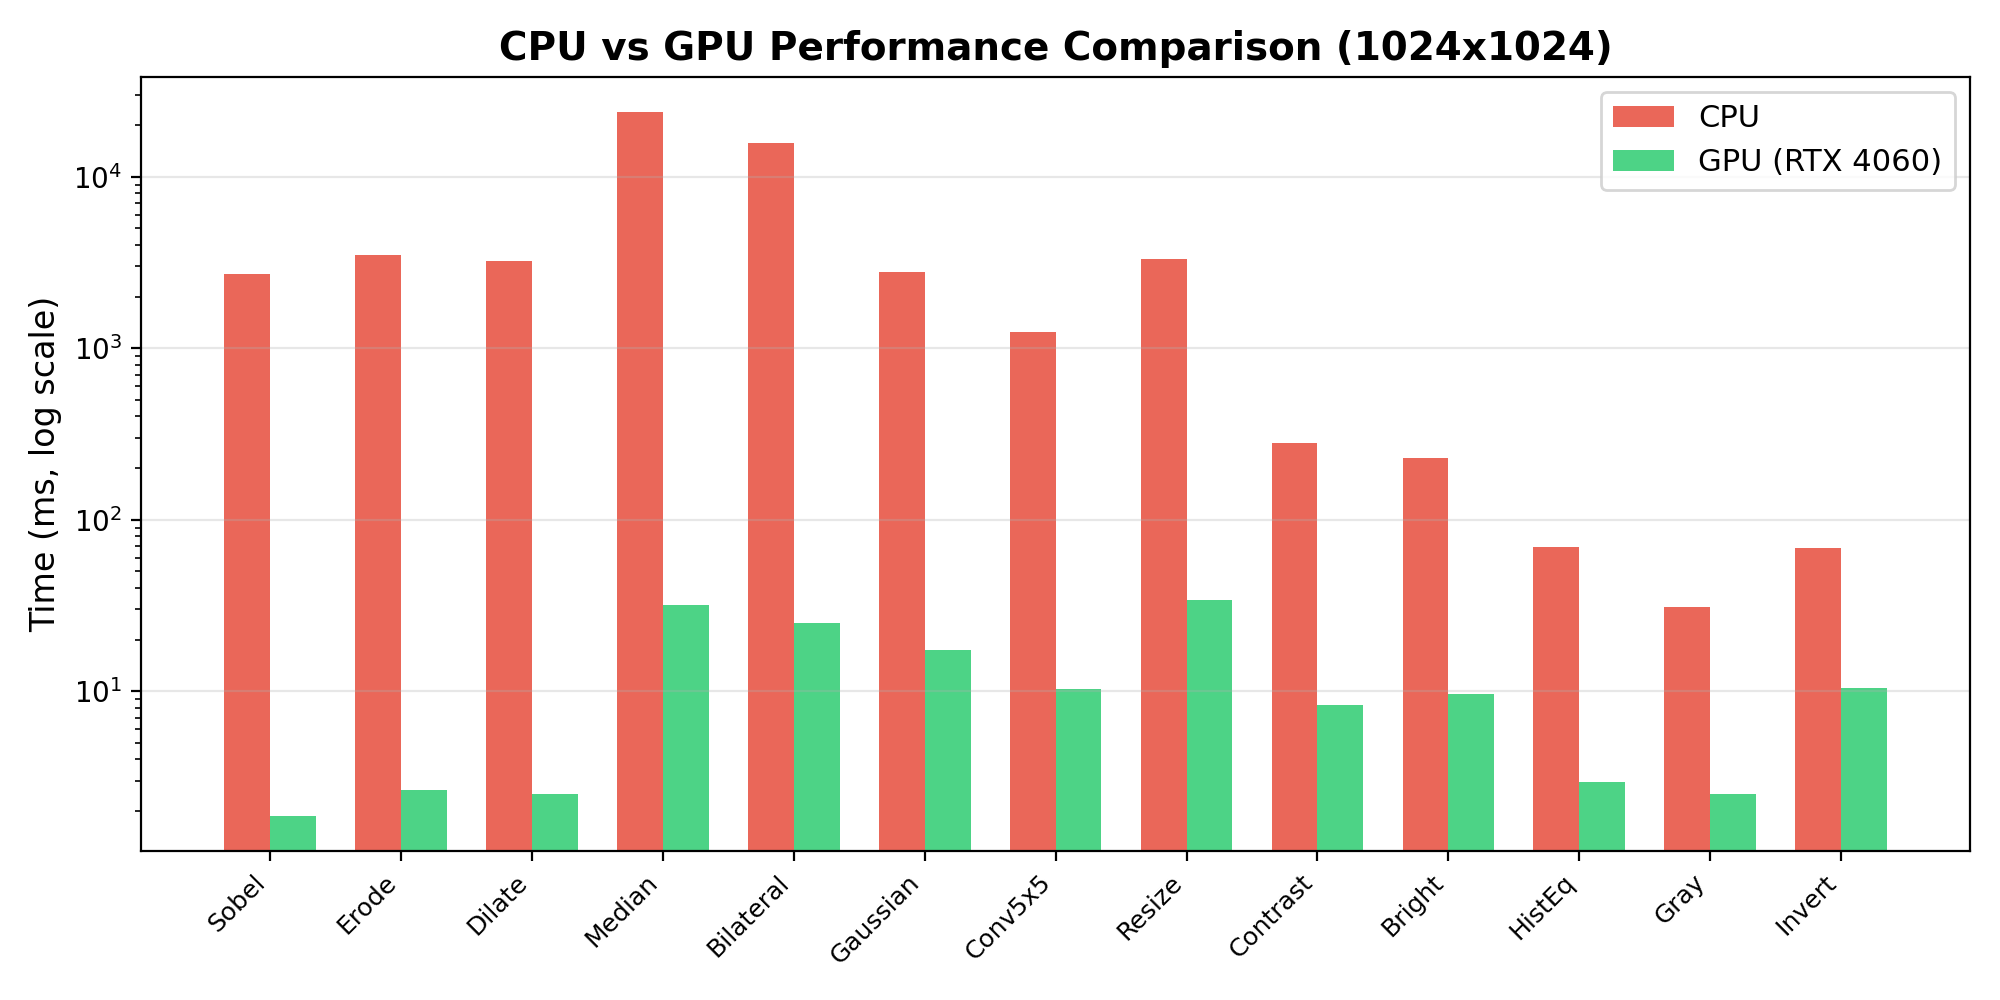
\includegraphics[width=\columnwidth]{figures/benchmark_bars.png}
            \caption{CPU vs GPU execution time comparison (log scale). The gap illustrates the orders-of-magnitude improvement achieved by CUDA parallelization.}
            \label{fig:benchmark}
        \end{figure}

    \subsection{Speedup Analysis}

        \figref{fig:speedup} presents the speedup factors for all benchmarked operations, color-coded by magnitude. \figref{fig:category} groups these results by operation category to reveal architectural insights.

        \begin{figure}[H]
            \centering
            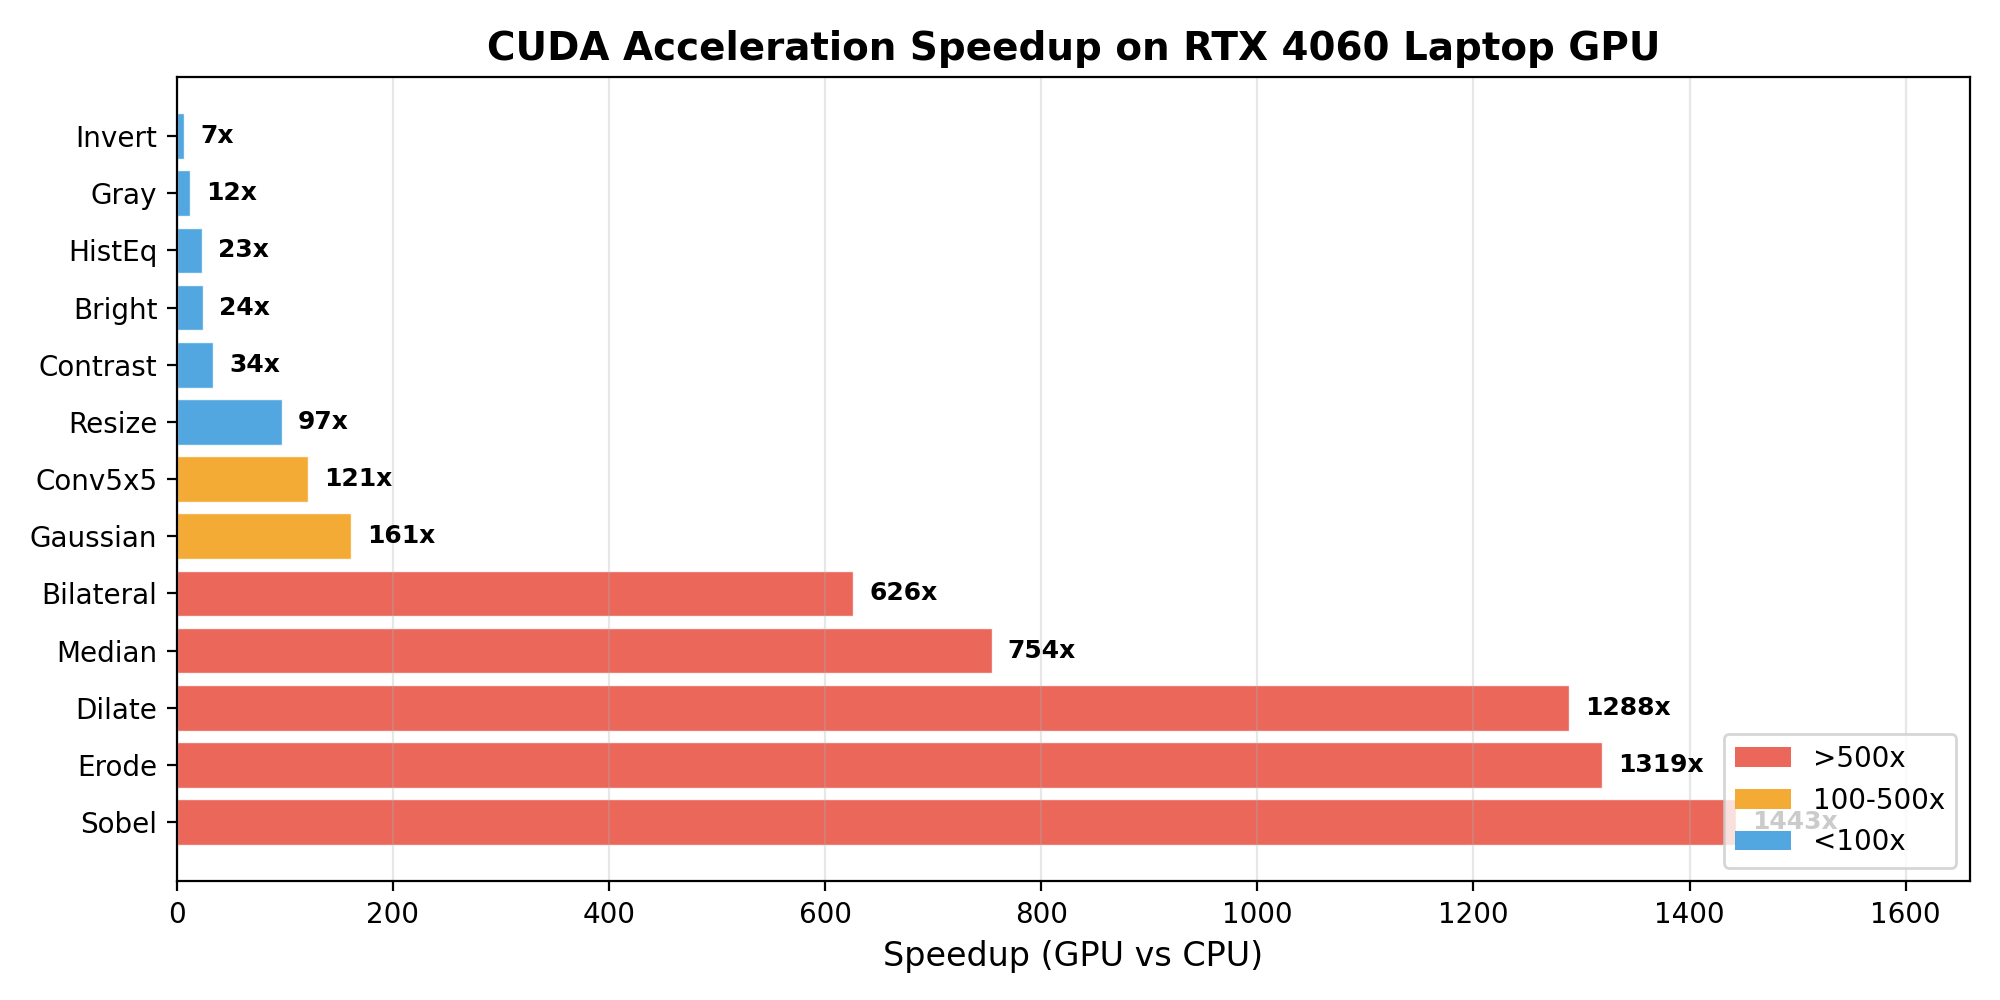
\includegraphics[width=\columnwidth]{figures/speedup_chart.png}
            \caption{CUDA acceleration speedup across all operations. Neighborhood operations (red) achieve >1000$\times$, non-linear filters (orange) >600$\times$, and per-pixel operations (blue) 7--34$\times$.}
            \label{fig:speedup}
        \end{figure}

        \begin{figure}[H]
            \centering
            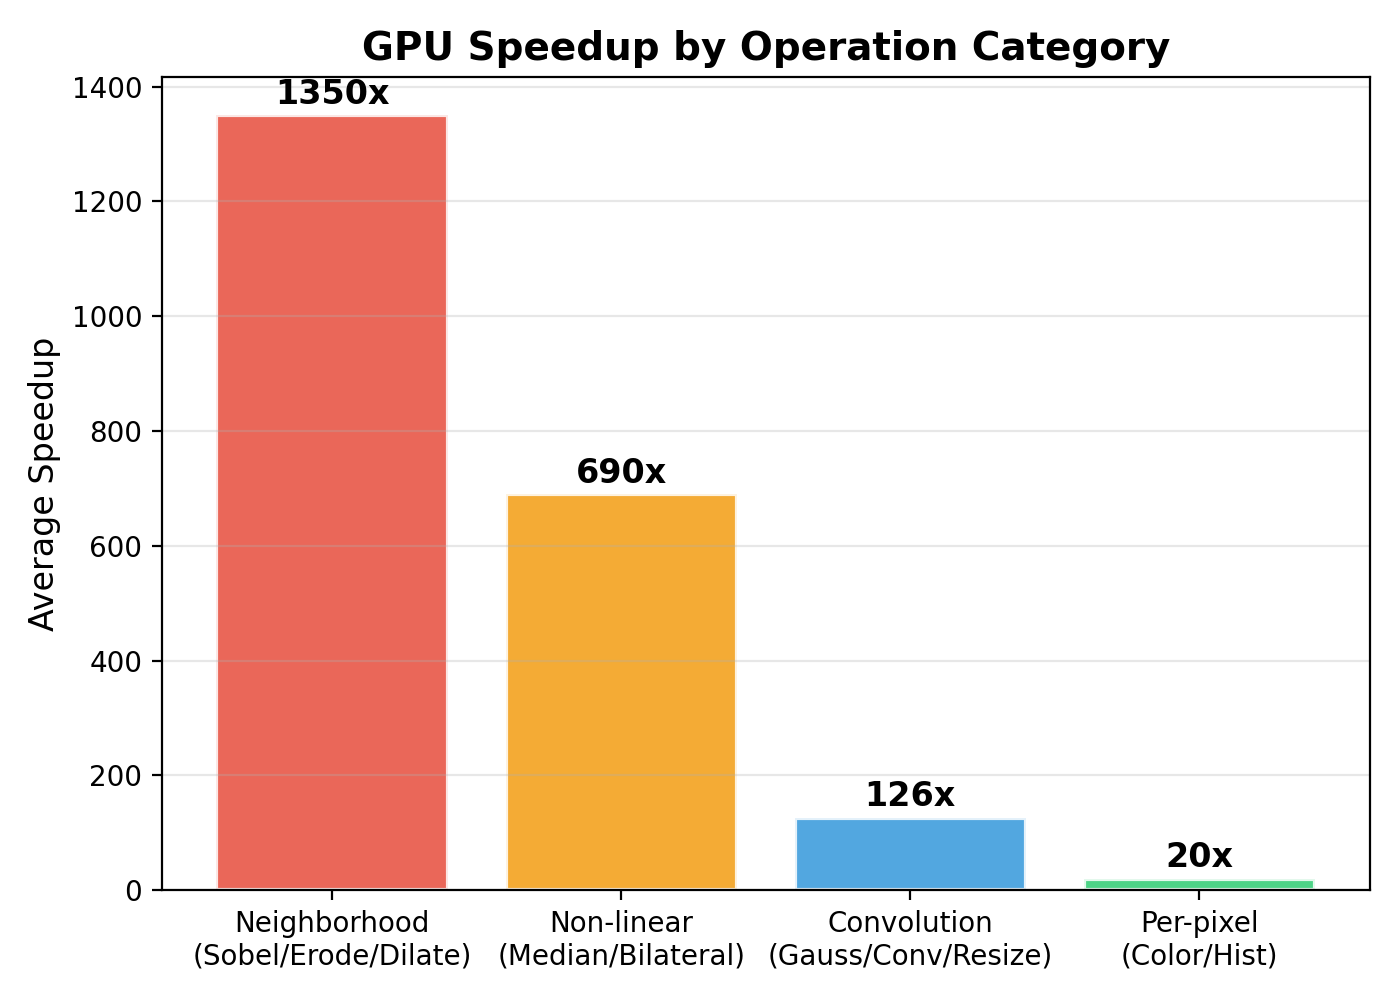
\includegraphics[width=0.85\columnwidth]{figures/category_speedup.png}
            \caption{Average GPU speedup grouped by operation category. Neighborhood operations benefit most from spatial parallelism and shared memory caching.}
            \label{fig:category}
        \end{figure}

        The results reveal several patterns:

        \begin{enumerate}
            \item \textbf{Neighborhood operations} (Sobel, erode/dilate) achieve the highest speedups (1000$\times$+) because each output pixel requires reading a spatial neighborhood -- a pattern ideally suited to GPU parallel execution with shared memory caching.
            \item \textbf{Non-linear filters} (median, bilateral) benefit enormously from GPU parallelism: the CPU must process each pixel sequentially with expensive sorting or exponential computations, while the GPU processes all pixels simultaneously.
            \item \textbf{Convolution-based operations} (Gaussian, generic convolution, resize) show 97--161$\times$ speedups, limited by the ratio of arithmetic to memory operations.
            \item \textbf{Per-pixel operations} (brightness, invert, grayscale) show moderate speedups (7--34$\times$) as they are memory-bandwidth-bound. The transfer overhead becomes a significant fraction of total time.
        \end{enumerate}

    \subsection{Pipeline Performance}

        \figref{fig:pipeline} compares a four-stage processing pipeline running on CPU versus GPU.

        \begin{figure}[H]
            \centering
            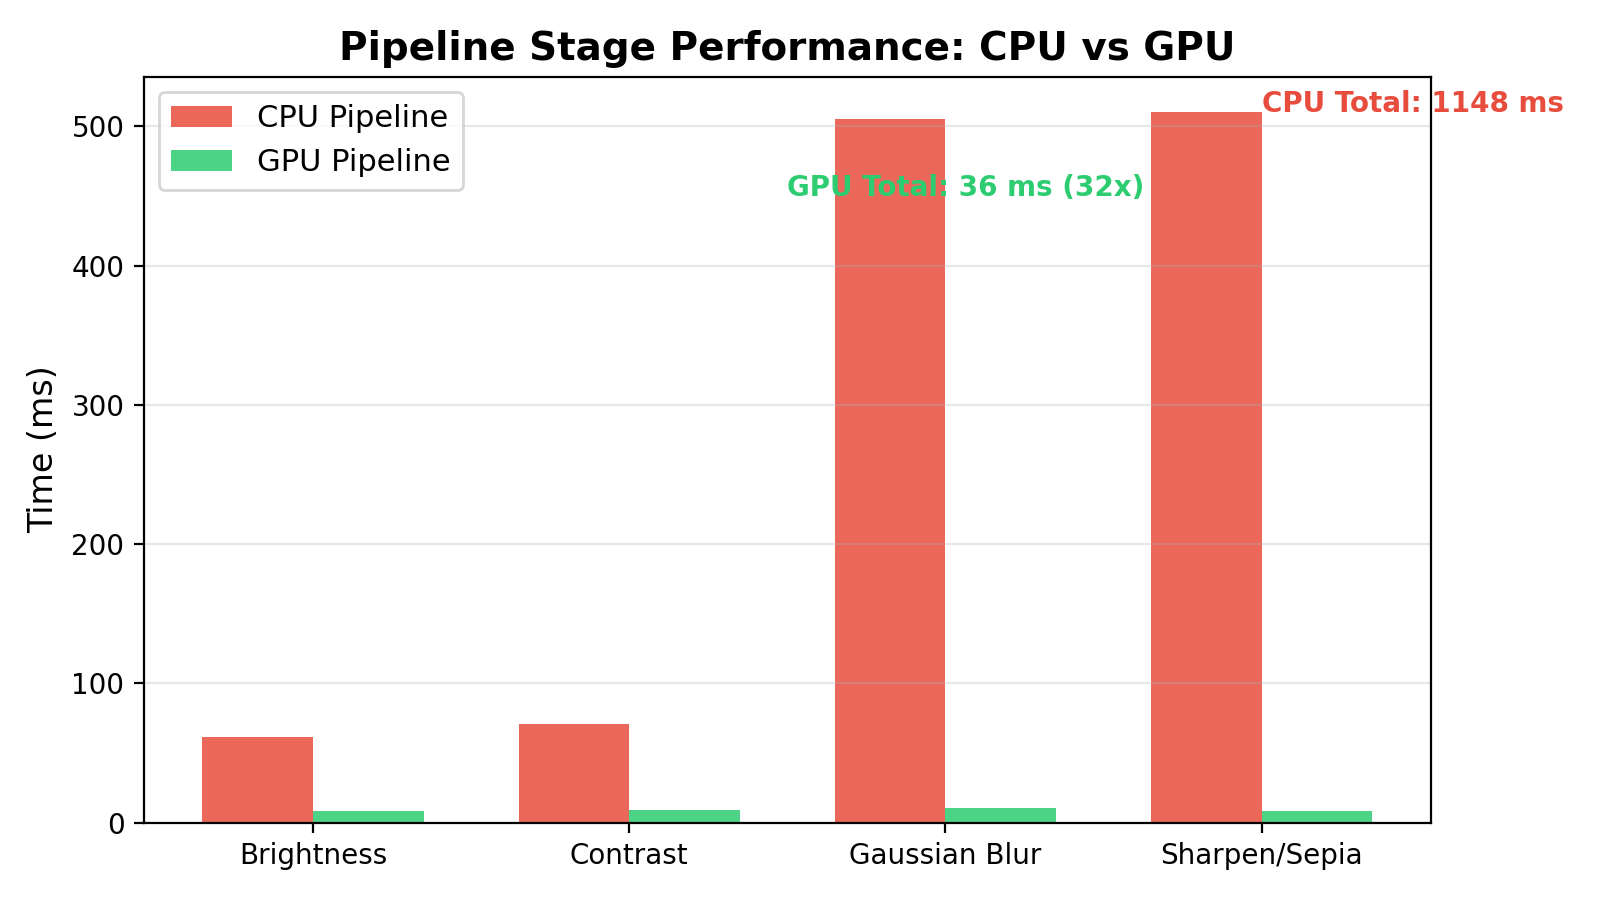
\includegraphics[width=0.85\columnwidth]{figures/pipeline_compare.png}
            \caption{Pipeline stage timing: CPU total 1,148 ms vs GPU total 36 ms. The GPU pipeline achieves a \textbf{32$\times$} end-to-end speedup.}
            \label{fig:pipeline}
        \end{figure}

        The GPU pipeline (brightness $\rightarrow$ contrast $\rightarrow$ Gaussian blur $\rightarrow$ sepia) completes in \textbf{36 ms} compared to \textbf{1,148 ms} on CPU, demonstrating consistent acceleration across chained operations.

\section{Software Engineering Practices}

    \subsection{Build System}

        The Visual Studio solution supports conditional CUDA compilation:
        \begin{itemize}
            \item When \texttt{IMAGELIB\_HAS\_CUDA} is defined and CudaLib is built, all GPU operations are available.
            \item Without CUDA, \texttt{GpuAccel.cpp} compiles stub implementations, ensuring the library remains functional on systems without NVIDIA GPUs.
        \end{itemize}

    \subsection{Plugin Architecture}

        The \texttt{Plugin} module provides an \texttt{IImagePlugin} interface supporting both lambda-based registration and DLL-based dynamic loading (via \texttt{LoadLibrary}/\texttt{GetProcAddress} on Windows). The \texttt{PluginManager} singleton maintains a registry of named plugins.

    \subsection{Processing Pipeline}

        The \texttt{Pipeline<T>} template enables fluent stage composition with built-in profiling. Each stage reports execution time via \texttt{executeWithProfile()}, facilitating performance analysis and bottleneck identification.

    \subsection{Thread Pool}

        A lock-based thread pool with \texttt{parallelFor} and \texttt{parallelFor2D} methods distributes work across available cores. The Mandelbrot benchmark demonstrates 24-core utilization, completing a 1024$\times$768 fractal in 41 ms.

\section{Conclusion}

    This project demonstrates that a modern C++ image processing library with CUDA acceleration can achieve performance gains of up to three orders of magnitude. Key achievements include:

    \begin{itemize}
        \item A \textbf{complete image processing toolkit} spanning 15 modules with 4,500+ lines of C++20 code and 80+ unit tests.
        \item \textbf{CUDA GPU acceleration} achieving up to \textbf{1,441$\times$} speedup on an RTX 4060, with 10 optimized kernel files employing shared memory tiling, constant memory, histogram-based parallel algorithms, and iterative convergence.
        \item \textbf{Clean architecture} separating CPU and GPU code across independent projects, with conditional compilation ensuring compatibility on non-CUDA systems.
        \item \textbf{Real-world pipeline performance}: 32$\times$ end-to-end speedup on a multi-stage image processing pipeline.
    \end{itemize}

    Future work could extend the library with deep learning integration (tensor operations), video processing support, multi-GPU scaling, and Vulkan compute shaders for cross-platform GPU acceleration.

%----------------------------------------------------------

\printbibliography

%----------------------------------------------------------

\end{document}
